\chapter{3D Model of the Parallelepiped}

As shown in the images, to enhance the understanding of the scene, I chose to colour the back wall of the parallelepiped black and render it empty. This decision was made to improve the visibility of the depth.

The recovered \verb|3D| model of the rectangular parallelepiped is displayed.

\begin{figure}[H]
     \centering
     \begin{subfigure}[b]{0.4\textwidth}
         \centering
         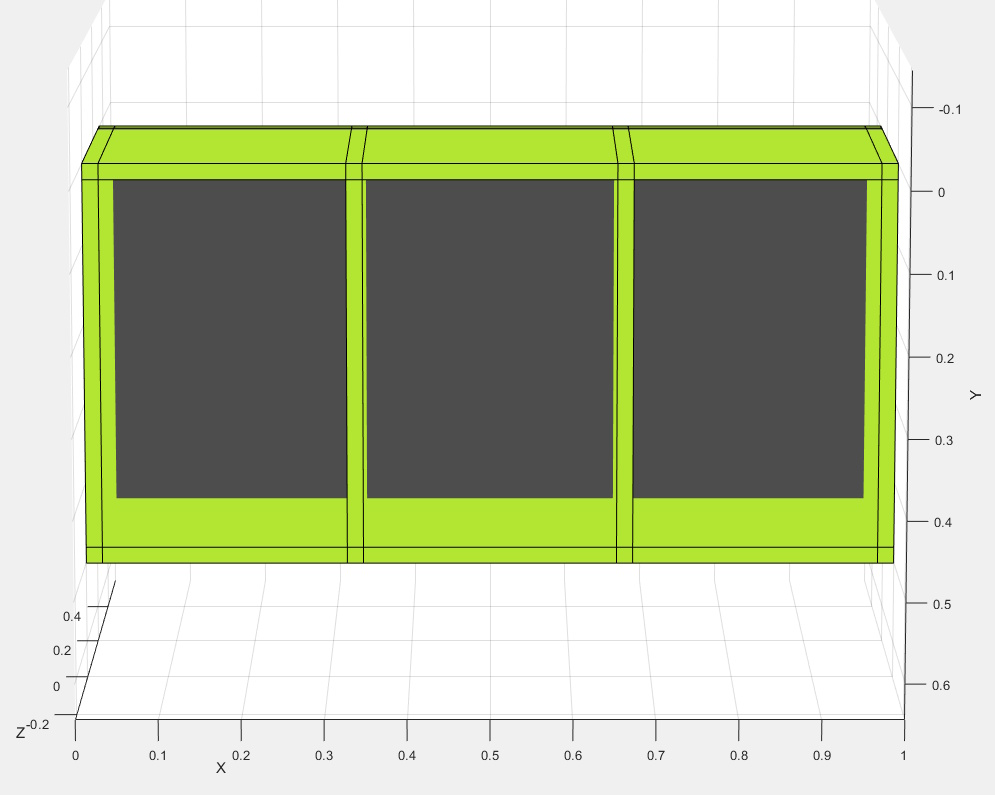
\includegraphics[width=\textwidth]{img/3d_1.jpg}
         \caption{3D model - View 1}
     \end{subfigure}
     \hfill
     \begin{subfigure}[b]{0.4\textwidth}
         \centering
         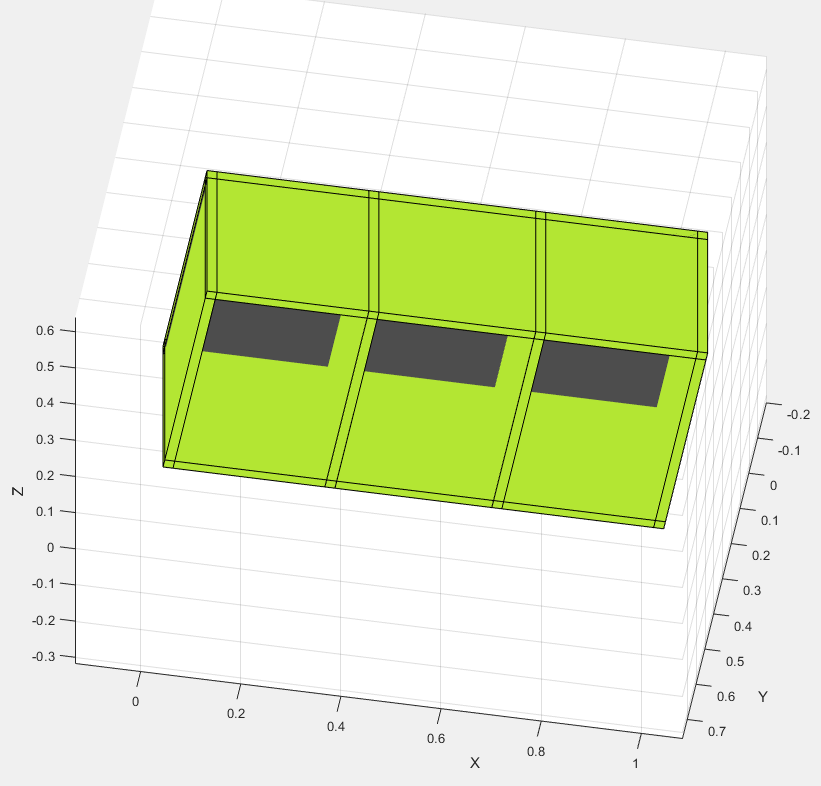
\includegraphics[width=\textwidth]{img/3d_3.jpg}
         \caption{3D model - View 2}
     \end{subfigure}
\end{figure}

\begin{figure}[H]
    \centering
    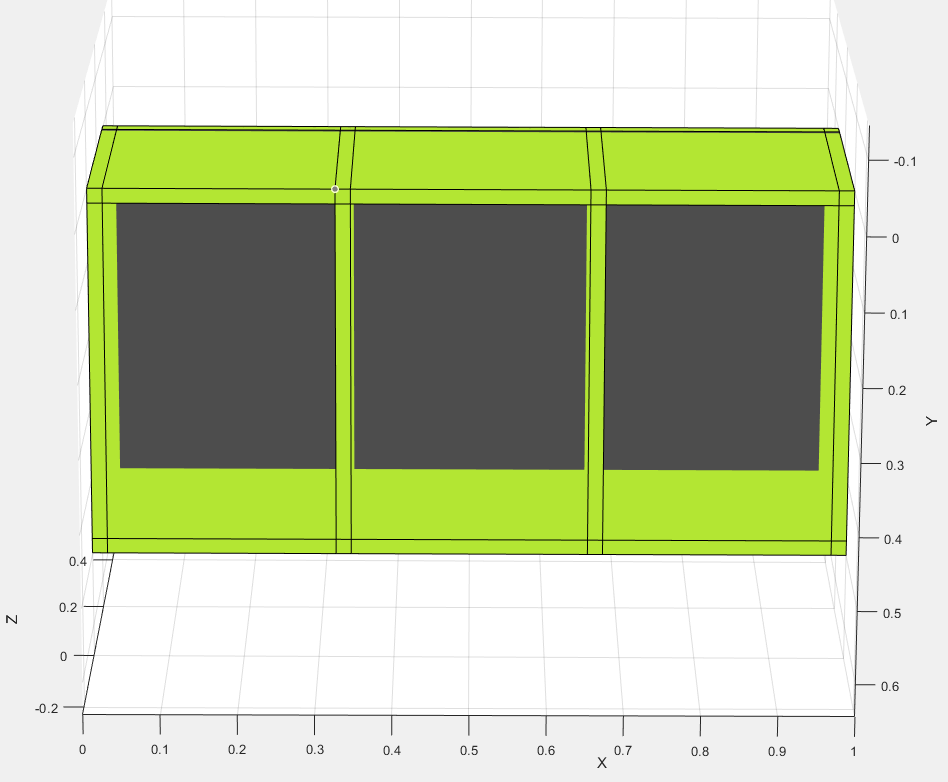
\includegraphics[width=0.5\linewidth]{img/3d_2.jpg}
    \caption{3D model - View 3}
\end{figure}